\documentclass[12pt]{book}
%\usepackage{pdf14}
%Paper saving
%\documentclass[12pt,openany]{book}
%\documentclass[10pt,openany]{book}
%\documentclass[8pt,openany]{extbook}


%See text for 
%FIXMEevillayouthack
% for evil layout hacks

%FIXME: Check the diagram in the preface in tex4ht
\usepackage{diffyqssetup}

\author{Ji\v{r}\'i Lebl}

\title{Notes on Diffy Qs: Differential Equations for Engineers}

% Set up our index
\makeindex

%mbx <!--BEFORE book-->

%mbxdocinfo    <website>
%mbxdocinfo        <title>www.jirka.org/diffyqs/</title>
%mbxdocinfo        <url>http://www.jirka.org/diffyqs/</url>
%mbxdocinfo    </website>
%mbxdocinfo
%mbxdocinfo    <initialism>DIFFYQS</initialism>


%mbxmacro \newcommand{\nicefrac}[2]{{{}^{#1}}\!/\!{{}_{#2}}}
%mbxmacro \newcommand{\unitfrac}[3][\!\!]{#1 \,\, {{}^{#2}}\!/\!{{}_{#3}}}
%mbxmacro \newcommand{\unit}[2][\!\!]{#1 \,\, #2}
%mbxmacro \newcommand{\noalign}[1]{}

\begin{document}

%mbx <title>Notes on Diffy Qs</title>
%mbx <subtitle>Differential Equations for Engineers</subtitle>
%mbx
%mbx <frontmatter>
%mbx   <titlepage>
%mbx
%mbx     <author>
%mbx       <personname>Jiří Lebl</personname>
%mbx       <department>Department of Mathematics</department>
%mbx       <institution>Oklahoma State University</institution>
%mbx       <email>jiri.lebl@gmail.com</email>
%mbx     </author>
%mbx
%mbx     <date><today /></date>
%mbx
%mbx   </titlepage>
%mbx
%mbx   <colophon>
%mbx
%mbx     <copyright>
%mbx       <year>2008<ndash />2017</year>
%mbx       <holder>Jiří Lebl</holder>
%mbx       <minilicense>FIXME License</minilicense>
%mbx       <shortlicense>FIXME</shortlicense>
%mbx     </copyright>
%mbx
%mbx   </colophon>
%mbx </frontmatter>

%mbxSTARTIGNORE

\newcommand{\theversion}{5.2}
\makediffytitlepage

\pagebreak

\vspace*{\fill}

%\begin{small} 
\noindent
Typeset in \LaTeX.

\bigskip

\noindent
Copyright \copyright 2008--2017 Ji\v{r}\'i Lebl

%\medskip
%\noindent
%Createspace edition\\
%ISBN-13: 978-1541329058

\bigskip

%\begin{floatingfigure}{1.4in}
%\vspace{-0.05in}
\noindent
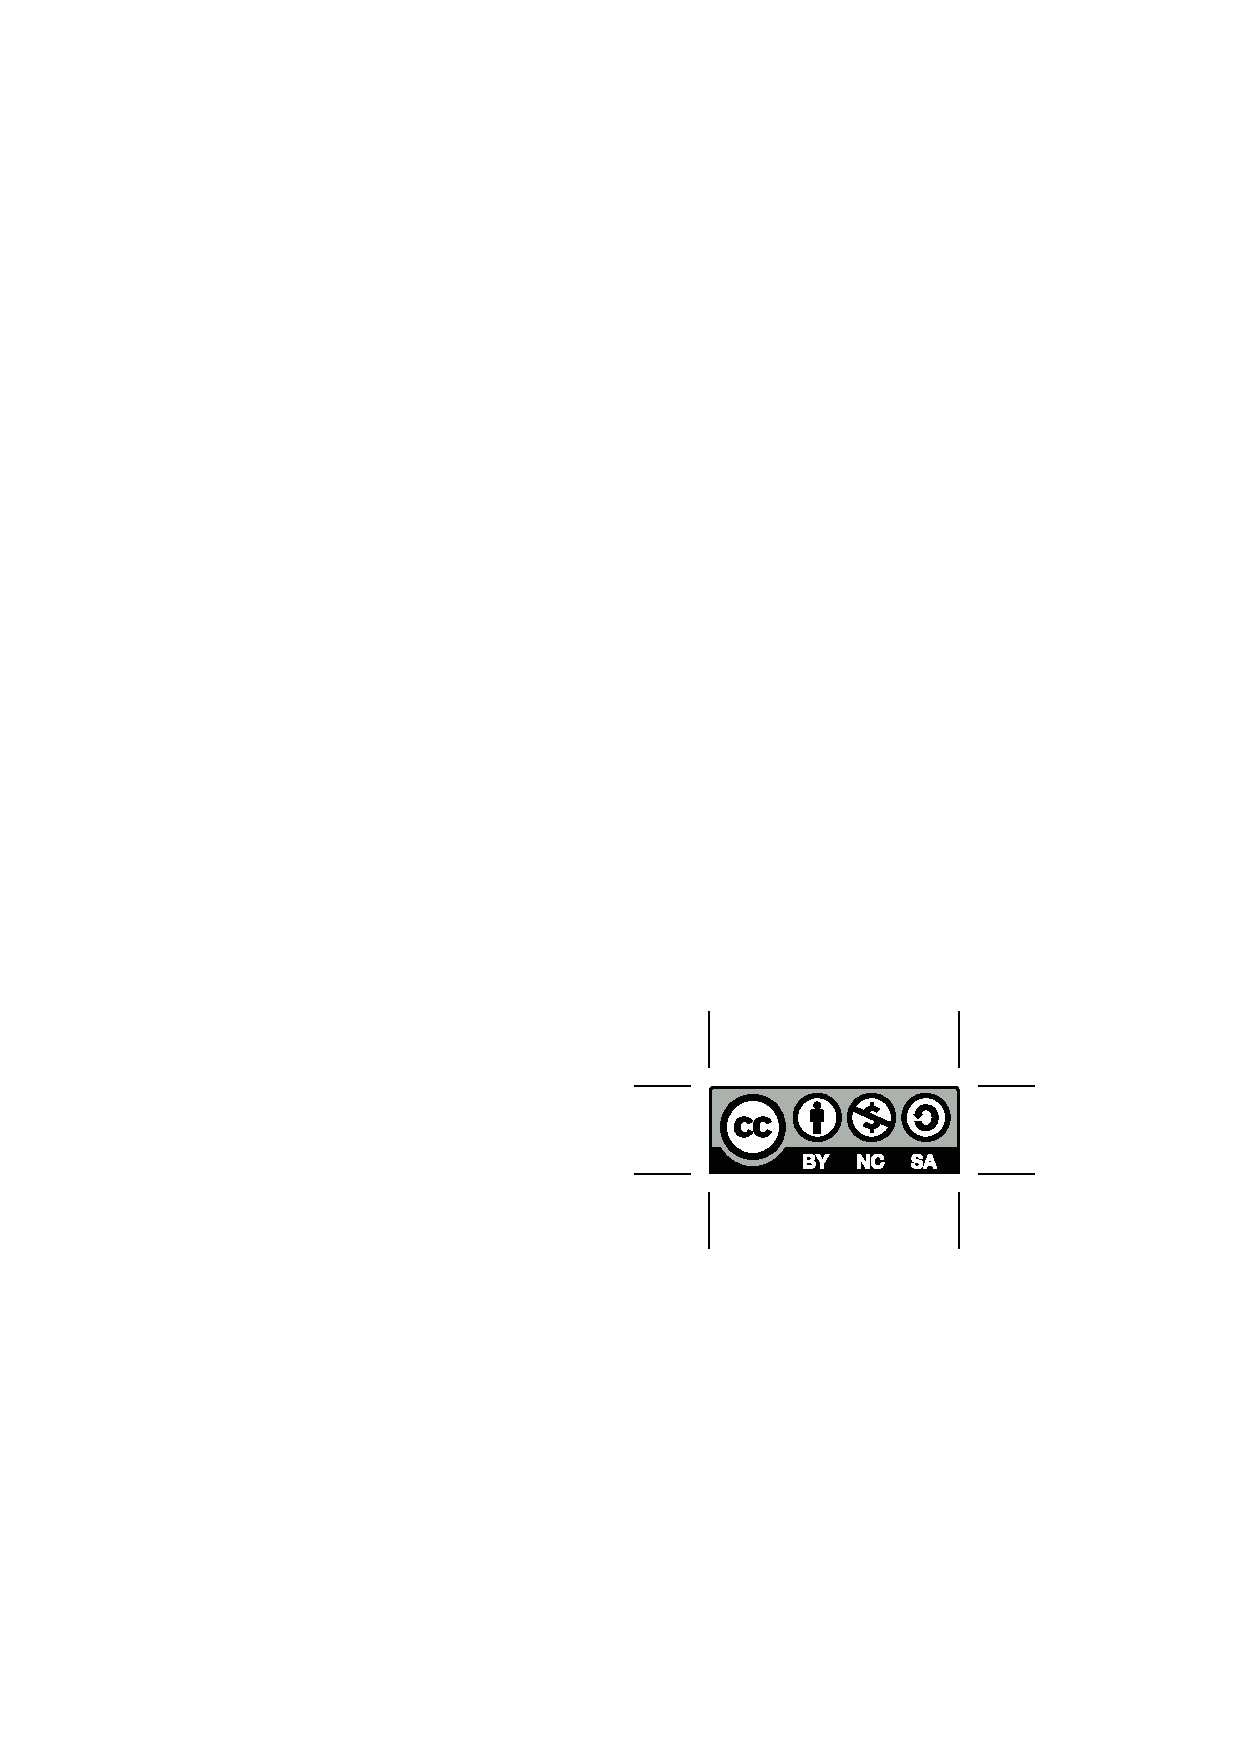
\includegraphics[width=1.38in]{figures/license}
\quad

\includegraphics[width=1.38in]{figures/license2}
%\end{floatingfigure}

\bigskip

\noindent
This work is dual licensed under
the Creative Commons
Attribution-Non\-commercial-Share Alike 4.0 International License and
the Creative Commons
Attribution-Share Alike 4.0 International License.
To view a
copy of these licenses, visit
\url{http://creativecommons.org/licenses/by-nc-sa/4.0/}
or
\url{http://creativecommons.org/licenses/by-sa/4.0/}
or send a letter to
Creative Commons
PO Box 1866, Mountain View, CA 94042, USA.
%Creative Commons, 171 Second Street, Suite 300, San Francisco, California,
%94105, USA.

\bigskip

\noindent
You can use, print, duplicate, share this book as much as you want.  You can
base your own notes on it and reuse parts if you keep the license the
same.  You can assume the license is either the CC-BY-NC-SA or CC-BY-SA,
whichever is compatible with what you wish to do, your derivative works must
use at least one of the licenses.
%If you plan to use it commercially (sell it for more than just
%duplicating cost), then you need to contact me and we will work something out.
%If you are printing a course pack for your students, then it is fine if the 
%duplication service is charging a fee for printing and selling the printed
%copy.  I consider that duplicating cost.

\bigskip

\noindent
During the writing of these notes, 
the author was in part supported by NSF grant DMS-0900885 and
DMS-1362337.

\bigskip

\noindent
The date is the main identifier of version.  The major version / edition
number is raised only if there have been substantial changes.
%, if only
%very minor changes or fixes are done only the minor version is raised.
Edition
number started at 5, that is, version 5.0, as it was not kept track of
before.
%The Createspace edition ISBN number identifies the major version, and is not
%changed for minor updates fixing errata.
%The edition given with the ISBN number is the major version.

\bigskip

\noindent
See \url{http://www.jirka.org/diffyqs/} for more information
(including contact information).
%\end{small}

% For large print do this
%\large

\diffytableofcontents

\newpage

%mbxENDIGNORE

%mbx <!--HERE IS WHERE WE ADD MBX PREAMBLE AFTER book-->
%mbx <!--HERE IS WHERE WE ADD MBX PREAMBLE 2-->

%%%%%%%%%%%%%%%%%%%%%%%%%%%%%%%%%%%%%%%%%%%%%%%%%%%%%%%%%%%%%%%%%%%%%%%%%%%%%%

% Introduction chapter
\input ch-intro.tex

%%%%%%%%%%%%%%%%%%%%%%%%%%%%%%%%%%%%%%%%%%%%%%%%%%%%%%%%%%%%%%%%%%%%%%%%%%%%%%

% First order ODEs chapter
\input ch-first-order-ode.tex

%%%%%%%%%%%%%%%%%%%%%%%%%%%%%%%%%%%%%%%%%%%%%%%%%%%%%%%%%%%%%%%%%%%%%%%%%%%%%%

% Higher order linear ODEs chapter
\input ch-higher-order-ode.tex

%%%%%%%%%%%%%%%%%%%%%%%%%%%%%%%%%%%%%%%%%%%%%%%%%%%%%%%%%%%%%%%%%%%%%%%%%%%%%%

% Systems of ODEs chapter
\input ch-systems.tex

%%%%%%%%%%%%%%%%%%%%%%%%%%%%%%%%%%%%%%%%%%%%%%%%%%%%%%%%%%%%%%%%%%%%%%%%%%%%%%

% Fourier series and PDEs chapter
\input ch-fourier-and-pde.tex

%%%%%%%%%%%%%%%%%%%%%%%%%%%%%%%%%%%%%%%%%%%%%%%%%%%%%%%%%%%%%%%%%%%%%%%%%%%%%%

% Eigenvalue problems chapter
\input ch-eigenvalue-probs.tex

%%%%%%%%%%%%%%%%%%%%%%%%%%%%%%%%%%%%%%%%%%%%%%%%%%%%%%%%%%%%%%%%%%%%%%%%%%%%%%

% The Laplace transform chapter
\input ch-laplace.tex

%%%%%%%%%%%%%%%%%%%%%%%%%%%%%%%%%%%%%%%%%%%%%%%%%%%%%%%%%%%%%%%%%%%%%%%%%%%%%%

% Power series methods chapter
\input ch-power-ser.tex

%%%%%%%%%%%%%%%%%%%%%%%%%%%%%%%%%%%%%%%%%%%%%%%%%%%%%%%%%%%%%%%%%%%%%%%%%%%%%%

% Nonlinear systems chapter
\input ch-nonlin-systems.tex

%%%%%%%%%%%%%%%%%%%%%%%%%%%%%%%%%%%%%%%%%%%%%%%%%%%%%%%%%%%%%%%%%%%%%%%%%%%%%%
%%%%%%%%%%%%%%%%%%%%%%%%%%%%%%%%%%%%%%%%%%%%%%%%%%%%%%%%%%%%%%%%%%%%%%%%%%%%%%
%%%%%%%%%%%%%%%%%%%%%%%%%%%%%%%%%%%%%%%%%%%%%%%%%%%%%%%%%%%%%%%%%%%%%%%%%%%%%%

%must be in separate "paragraph"
%mbxBACKMATTER

%mbx <backmatter>

%%%%%%%%%%%%%%%%%%%%%%%%%%%%%%%%%%%%%%%%%%%%%%%%%%%%%%%%%%%%%%%%%%%%%%%%%%%%%%
%%%%%%%%%%%%%%%%%%%%%%%%%%%%%%%%%%%%%%%%%%%%%%%%%%%%%%%%%%%%%%%%%%%%%%%%%%%%%%
%%%%%%%%%%%%%%%%%%%%%%%%%%%%%%%%%%%%%%%%%%%%%%%%%%%%%%%%%%%%%%%%%%%%%%%%%%%%%%

%mbxSTARTIGNORE

%FIXME: This makes contents fit
\addextraspacetotoc

\renewcommand{\bibname}{Further Reading}

\begin{thebibliography}{MM}

\addfakecontentsline{Further Reading}

\label{furtherreading:chapter}

\bibitem[BM]{BM}
 Paul W.\ Berg and James L.\ McGregor, 
 \emph{\href{http://books.google.com/books?id=EfJQAAAAMAAJ}{Elementary
Partial Differential Equations}}, 
 Holden-Day,
 San Francisco, CA,
 1966.

\bibitem[BD]{BD}
 William E.\ Boyce and
 Richard C.\ DiPrima,
 \emph{\href{http://books.google.com/books?id=nYWcQgAACAAJ}{Elementary
Differential Equations and Boundary Value Problems}},
 9th edition,
 John Wiley \& Sons Inc.,
 New York, NY, 2008.

\bibitem[EP]{EP}
 C.H.\ Edwards and D.E.\ Penney,
 \emph{\href{http://books.google.com/books?id=qi6ePwAACAAJ}{Differential
Equations and Boundary Value Problems: Computing and Modeling}},
 4th edition,
 Prentice Hall,
 2008.

\bibitem[F]{F}
 Stanley J.\ Farlow,
 \emph{\href{http://books.google.com/books?id=_ozWAAAAMAAJ}{An Introduction
to Differential Equations and Their Applications}},
 McGraw-Hill, Inc.,
 Princeton, NJ,
 1994.  (Published also by Dover Publications, 2006.)

\bibitem[I]{I}
 E.L.\ Ince,
 \emph{\href{http://books.google.com/books?id=uYz-pqUD75gC}{Ordinary
Differential Equations}},
 Dover Publications, Inc.,
 New York, NY,
 1956.

\bibitem[T]{T}
 William F.\ Trench,
 \emph{Elementary Differential Equations with Boundary Value
Problems}. Books and Monographs. Book 9.  2013.
\url{http://digitalcommons.trinity.edu/mono/9}

\end{thebibliography}
%mbxENDIGNORE

%mbx <references xml:id="furtherreading_chapter">
%mbx   <title>Further Reading</title>
%mbx
%mbx   <biblio type="raw" xml:id="biblio-BM" tag="BM">Paul W. Berg and
%mbx     James L. McGregor, 
%mbx     <title><url href="http://books.google.com/books?id=EfJQAAAAMAAJ"
%mbx     >Elementary Partial Differential Equations</url></title>,
%mbx     Holden-Day, San Francisco, CA, 1966.</biblio>
%mbx
%mbx   <biblio type="raw" xml:id="biblio-BD" tag="BD">William E. Boyce and
%mbx     Richard C. DiPrima,
%mbx     <title><url href="http://books.google.com/books?id=nYWcQgAACAAJ"
%mbx     >Elementary Differential Equations and Boundary Value
%mbx     Problems</url></title>,
%mbx     9th edition, John Wiley &amp; Sons Inc., New York, NY, 2008.</biblio>
%mbx
%mbx   <biblio type="raw" xml:id="biblio-EP" tag="EP">C.H. Edwards
%mbx     and D.E. Penney,
%mbx     <title><url href="http://books.google.com/books?id=qi6ePwAACAAJ"
%mbx     >Differential Equations and Boundary Value Problems: Computing and
%mbx     Modeling</url></title>,
%mbx     4th edition, Prentice Hall, 2008.</biblio>
%mbx
%mbx   <biblio type="raw" xml:id="biblio-F" tag="F">Stanley J. Farlow,
%mbx     <title><url href="http://books.google.com/books?id=_ozWAAAAMAAJ"
%mbx     >An Introduction to Differential Equations and Their
%mbx     Applications</url></title>,
%mbx     McGraw-Hill, Inc., Princeton, NJ, 1994.  (Published also by Dover
%mbx     Publications, 2006.)</biblio>
%mbx
%mbx   <biblio type="raw" xml:id="biblio-I" tag="I">E.L. Ince,
%mbx     <title><url href="http://books.google.com/books?id=uYz-pqUD75gC"
%mbx     >Ordinary Differential Equations</url></title>,
%mbx     Dover Publications, Inc., New York, NY, 1956.</biblio>
%mbx
%mbx   <biblio type="raw" xml:id="biblio-T" tag="T">William F. Trench,
%mbx     <title>Elementary Differential Equations with Boundary Value
%mbx     Problems</title>, Books and Monographs, Book 9,  2013,
%mbx     <url>http://digitalcommons.trinity.edu/mono/9</url>.</biblio>
%mbx
%mbx </references>



%%%%%%%%%%%%%%%%%%%%%%%%%%%%%%%%%%%%%%%%%%%%%%%%%%%%%%%%%%%%%%%%%%%%%%%%%%%%%%
%%%%%%%%%%%%%%%%%%%%%%%%%%%%%%%%%%%%%%%%%%%%%%%%%%%%%%%%%%%%%%%%%%%%%%%%%%%%%%
%%%%%%%%%%%%%%%%%%%%%%%%%%%%%%%%%%%%%%%%%%%%%%%%%%%%%%%%%%%%%%%%%%%%%%%%%%%%%%

%mbxSTARTIGNORE
\printanswers
%mbxENDIGNORE

%%%%%%%%%%%%%%%%%%%%%%%%%%%%%%%%%%%%%%%%%%%%%%%%%%%%%%%%%%%%%%%%%%%%%%%%%%%%%%
%%%%%%%%%%%%%%%%%%%%%%%%%%%%%%%%%%%%%%%%%%%%%%%%%%%%%%%%%%%%%%%%%%%%%%%%%%%%%%
%%%%%%%%%%%%%%%%%%%%%%%%%%%%%%%%%%%%%%%%%%%%%%%%%%%%%%%%%%%%%%%%%%%%%%%%%%%%%%

%mbxSTARTIGNORE
\diffyindex
%mbxENDIGNORE

%mbx   <index>
%mbx     <title>Index</title>
%mbx     <index-list />
%mbx   </index>

%%%%%%%%%%%%%%%%%%%%%%%%%%%%%%%%%%%%%%%%%%%%%%%%%%%%%%%%%%%%%%%%%%%%%%%%%%%%%%
%%%%%%%%%%%%%%%%%%%%%%%%%%%%%%%%%%%%%%%%%%%%%%%%%%%%%%%%%%%%%%%%%%%%%%%%%%%%%%
%%%%%%%%%%%%%%%%%%%%%%%%%%%%%%%%%%%%%%%%%%%%%%%%%%%%%%%%%%%%%%%%%%%%%%%%%%%%%%

%mbx </backmatter>

\end{document}

